% c4-treeclock-v.tex

\documentclass{standalone}
% newcommands.tex

\usepackage{amssymb, latexsym}
\usepackage{bbding} % for checkmark and xsolid
\usepackage{mathtools}

% math
\newcommand{\N}{\mathbb{N}}
\newcommand{\set}[1]{\{#1\}}
\newcommand{\bset}[1]{\big\{#1\big\}}
\newcommand{\ps}{\mathcal{P}} % for powerset
\newcommand{\emptyseq}{\emptyset} % or using <>?
\newcommand{\tuple}[1]{\langle#1\rangle} % or using (#1)?
\newcommand{\btuple}[1]{\big\langle#1\big\rangle}

\newcommand{\post}{\mathit{post}}
\newcommand{\comment}{\mathit{comment}}
\newcommand{\emptypost}{\mathit{empty}}
\newcommand{\acct}{\brown{\mathit{acct}}}

\newcommand{\yes}{\green{\Checkmark}}
\newcommand{\no}{\red{\XSolidBrush}}

\newcommand{\Key}{{\sf Key}}
\newcommand{\Val}{{\sf Val}}

\newcommand{\h}{\mathcal{H}}
%%%%%%%%%%%%%%% system models %%%%%%%%%%%%%%%
\newcommand{\E}{E}
\newcommand{\evar}{\mathit{e}}
\newcommand{\fvar}{\mathit{f}}
\newcommand{\Event}{{\sf Event}}
\newcommand{\REvent}{{\sf REvent}}
\newcommand{\WEvent}{{\sf WEvent}}
\newcommand{\HEvent}{{\sf HEvent}}
\newcommand{\op}{{\sf op}}
\newcommand{\Op}{{\sf Op}}
\newcommand{\opvar}{\mathit{op}}
\newcommand{\readevent}{{\sf R}}
\newcommand{\Read}{{\sf Read}\;}
\newcommand{\writeevent}{{\sf W}}
\newcommand{\Write}{{\sf Write}\;}
\newcommand{\WriteTx}{{\sf WriteTx}}
\newcommand{\W}{{\sf W}}
\newcommand{\R}{{\sf R}}
\newcommand{\T}{T}
%%%%%%%%%%%%%%% system models %%%%%%%%%%%%%%%

%%%%%%%%%%%%%%% axioms %%%%%%%%%%%%%%%
\renewcommand{\ae}{\mathcal{A}}
\newcommand{\axiom}{\Phi}
\newcommand{\rel}[1]{\xrightarrow{#1}}
\newcommand{\comp}{\;;\;}
\newcommand{\po}{{\sf po}}
\newcommand{\so}{\textsc{so}}
\newcommand{\rb}{\textsc{rb}}
\newcommand{\cb}{\textsc{cb}}
\newcommand{\vis}{\textsc{vis}}
\newcommand{\ar}{\textsc{ar}}
\newcommand{\hist}{\text{Hist}}
\newcommand{\intaxiom}{\textsc{Int}}
\newcommand{\extaxiom}{\textsc{Ext}}
\newcommand{\sessionaxiom}{\textsc{Session}}
\newcommand{\prefixaxiom}{\textsc{Prefix}}
\newcommand{\rbaxiom}{\textsc{ReturnBefore}}
\newcommand{\cbaxiom}{\textsc{CommitBefore}}
\newcommand{\conflict}{\bowtie}
\newcommand{\noconflictaxiom}{\textsc{NoConflict}}
\newcommand{\realtimesnapshotaxiom}{\textsc{RealtimeSnapshot}}
%%%%%%%%%%%%%%% axioms %%%%%%%%%%%%%%%

%%%%%%%%%%%%%%% consistency models %%%%%%%%%%%%%%%
\newcommand{\si}{\textsc{SI}}
\newcommand{\ansisi}{\textsc{ANSI-SI}}
\newcommand{\rtsi}{\textsc{RealtimeSI}}
\newcommand{\gsi}{\textsc{GSI}}
\newcommand{\parallelsi}{\textsc{PSI}}
\newcommand{\pcsi}{\textsc{PCSI}}
\newcommand{\strongsi}{\textsc{StrongSI}}
\newcommand{\strongsessionsi}{\textsc{SI}} % StrongSessionSI
\newcommand{\sessionsi}{\textsc{SessionSI}}
\newcommand{\nmsi}{\textsc{NMSI}}
\newcommand{\ser}{\textsc{SER}}
%%%%%%%%%%%%%%% consistency models %%%%%%%%%%%%%%%

%%%%%%%%%%%%%%% pseudo-code %%%%%%%%%%%%%%%
\newcommand{\g}{G}
\newcommand{\inducedgraph}{I}
\newcommand{\eithervar}{\mathit{either}}
\newcommand{\orvar}{\mathit{or}}
\newcommand{\reachability}{\textsc{Reachability}}
\newcommand{\reachabilityvar}{\mathit{reachability}}

\newcommand{\vertex}{\mathsf{Vertex}}
\newcommand{\edges}{\mathsf{Edge}}
\newcommand{\cons}{\mathsf{Cons}}

\newcommand{\vvar}{\mathit{v}}
\newcommand{\precvar}{\mathit{prec}}
\newcommand{\egvar}{\mathit{e}}
\newcommand{\edgevar}{\mathit{edge}}
\newcommand{\cvar}{\mathit{c}}
\newcommand{\consvar}{\mathit{cons}}

\newcommand{\BV}{\mathsf{BV}}
\newcommand{\Clause}{\mathsf{Cl}}
\newcommand{\DV}{\mathsf{DV}}
\newcommand{\formula}{\mathcal{F}}

\newcommand{\fromvar}{\mathit{from}}
\newcommand{\tovar}{\mathit{to}}
\newcommand{\typevar}{\mathit{type}}

\newcommand{\graphA}{\mathit{Dep}}
\newcommand{\graphB}{\mathit{AntiDep}}
\newcommand{\knowninducedgraph}{\mathit{KI}}
%%%%%%%%%%%%%%% pseudo-code %%%%%%%%%%%%%%%

%%%%%%%%%%%%%%% proof %%%%%%%%%%%%%%%
\newcommand{\inv}{\textsc{Inv}\;}
\newcommand{\case}{\textsc{Case}}
\newcommand{\casei}{\case\; I}
\newcommand{\caseii}{\case\; II}
%%%%%%%%%%%%%%% proof %%%%%%%%%%%%%%%

%%%%%%%%%%%%%%% checking %%%%%%%%%%%%%%%
\providecommand{\G}{}
\renewcommand{\G}{\mathcal{G}}
\renewcommand{\H}{\mathcal{H}}

\newcommand{\SO}{\textsf{SO}}
\newcommand{\WR}{\textsf{WR}}
\newcommand{\WW}{\textsf{WW}}
\newcommand{\RW}{\textsf{RW}}
%%%%%%%%%%%%%%% checking %%%%%%%%%%%%%%%

% colors
\newcommand{\red}[1]{\textcolor{red}{#1}}
\newcommand{\green}[1]{\textcolor{green}{#1}}
\newcommand{\blue}[1]{\textcolor{blue}{#1}}
\newcommand{\cyan}[1]{\textcolor{cyan}{#1}}
\newcommand{\brown}[1]{\textcolor{brown}{#1}}
\newcommand{\teal}[1]{\textcolor{teal}{#1}}
\newcommand{\purple}[1]{\textcolor{purple}{#1}}

\newcommand{\cobra}{\textsc{Cobra}}

\newcommand{\keyxvar}{\textcolor{cyan}{\mathit{x}}}
\newcommand{\keyyvar}{\textcolor{brown}{\mathit{y}}}

\usepackage{tikz}
\usetikzlibrary{calc, shapes, positioning, arrows.meta, decorations.pathmorphing}

\newlength{\sodist}
\newlength{\wrdist}
\setlength{\sodist}{0.60cm}
\setlength{\wrdist}{1.20cm}

\begin{document}
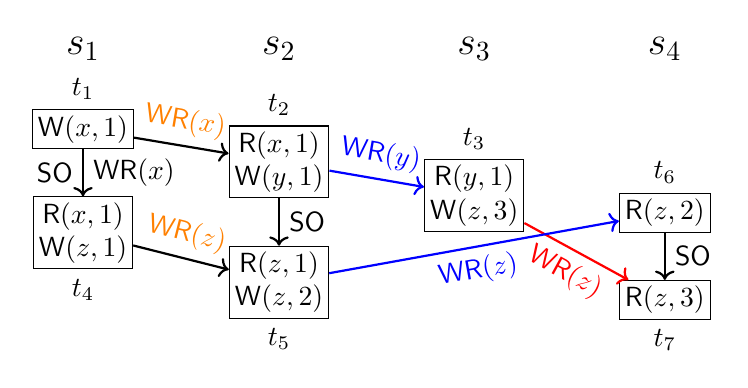
\begin{tikzpicture}[
  so/.style = {->, thick},
  wr/.style = {->, thick},
  co/.style = {->, thick},
  vo/.style = {->, thick},
  txn/.style = {draw, inner sep = 2pt}]

  % t1: W(x, 1)
  \node[txn, label = above : $t_{1}$]
		(t1) {$\writeevent(x, 1)$};
  % t4: R(x, 1) W(z, 1)
  \node[txn, below = \sodist of t1, label = below : $t_{4}$, align = center]
    (t4) {$\readevent(x, 1)$\\$\writeevent(z, 1)$};

  % t2: R(x, 1) W(y, 1)
  \node[txn, below right = -0.30cm and \wrdist of t1,
    label = above : $t_{2}$, align = center]
    (t2) {$\readevent(x, 1)$\\$\writeevent(y, 1)$};
	% t5: R(z, 1) W(z, 2)
  \node[txn, below = \sodist of t2, label = below : $t_{5}$, align = center]
    (t5) {$\readevent(z, 1)$\\$\writeevent(z, 2)$};

  % t3: R(y, 1) W(z, 3)
  \node[txn, below right = -0.50cm and \wrdist of t2,
    label = above : $t_{3}$, align = center]
    (t3) {$\readevent(y, 1)$\\$\writeevent(z, 3)$};

	% t6: R(z, 2)
  \node[txn, below right = -0.50cm and \wrdist of t3,
    label = above : $t_{6}$]
    (t6) {$\readevent(z, 2)$};
	% t7: R(z, 3)
  \node[txn, below = \sodist of t6, label = below : $t_{7}$]
    (t7) {$\readevent(z, 3)$};

	% session s1
	\node[above = 0.50cm of t1, font = \Large] (s1) {$s_{1}$};
  \node[font = \Large] (s2) at ($(s1 -| t2)$) {$s_{2}$};
  \node[font = \Large] (s3) at ($(s1 -| t3)$) {$s_{3}$};
  \node[font = \Large] (s4) at ($(s1 -| t6)$) {$s_{4}$};

  % t1-SO-t4
  \draw[so] (t1) to node[left]{$\SO$} node[right]{$\WR(x)$} (t4);
	% t2-SO-t5
  \draw[so] (t2) to node[right]{$\SO$} (t5);
	% t6-SO-t7
  \draw[so] (t6) to node[right]{$\SO$} (t7);

	% t1-t2-t3-t7
	\draw[wr] (t1) to node[sloped, above, orange] {$\WR(x)$} (t2);
	\draw[wr, blue] (t2) to node[sloped, above] {$\WR(y)$} (t3);
	\draw[wr, red] (t3) to node[sloped, below] {$\WR(z)$} (t7);

	% t4-t5-t6
	\draw[wr] (t4) to node[sloped, above, orange] {$\WR(z)$} (t5);
	\draw[wr, blue] (t5) to node[sloped, below] {$\WR(z)$} (t6);
\end{tikzpicture}
\end{document}